% TODO:
% 1) сделать пример после слайда ``Итератор'' как происходит обработка записей, как они проходят узлы

%%%%%%%%%%%%%%%%%%%%%%%%%%%%%%%%%%%%%%%%%
% Beamer Presentation
% LaTeX Template
% Version 1.0 (10/11/12)
%
% This template has been downloaded from:
% http://www.LaTeXTemplates.com
%
% License:
% CC BY-NC-SA 3.0 (http://creativecommons.org/licenses/by-nc-sa/3.0/)
%
%%%%%%%%%%%%%%%%%%%%%%%%%%%%%%%%%%%%%%%%%

%----------------------------------------------------------------------------------------
%	PACKAGES AND THEMES
%----------------------------------------------------------------------------------------

\documentclass{beamer}

\mode<presentation> {

% The Beamer class comes with a number of default slide themes
% which change the colors and layouts of slides. Below this is a list
% of all the themes, uncomment each in turn to see what they look like.

%\usetheme{default}
%\usetheme{AnnArbor}
%\usetheme{Antibes}
%\usetheme{Bergen}
%\usetheme{Berkeley}
%\usetheme{Berlin}
%\usetheme{Boadilla}
%\usetheme{CambridgeUS}
%\usetheme{Copenhagen}
%\usetheme{Darmstadt}
%\usetheme{Dresden}
%\usetheme{Frankfurt}
%\usetheme{Goettingen}
%\usetheme{Hannover}
%\usetheme{Ilmenau}
%\usetheme{JuanLesPins}
%\usetheme{Luebeck}
\usetheme{Madrid}
%\usetheme{Malmoe}
%\usetheme{Marburg}
%\usetheme{Montpellier}
%\usetheme{PaloAlto}
%\usetheme{Pittsburgh}
%\usetheme{Rochester}
%\usetheme{Singapore}
%\usetheme{Szeged}
%\usetheme{Warsaw}

% As well as themes, the Beamer class has a number of color themes
% for any slide theme. Uncomment each of these in turn to see how it
% changes the colors of your current slide theme.

%\usecolortheme{albatross}
%\usecolortheme{beaver}
%\usecolortheme{beetle}
%\usecolortheme{crane}
%\usecolortheme{dolphin}
%\usecolortheme{dove}
%\usecolortheme{fly}
%\usecolortheme{lily}
%\usecolortheme{orchid}
%\usecolortheme{rose}
%\usecolortheme{seagull}
%\usecolortheme{seahorse}
%\usecolortheme{whale}
%\usecolortheme{wolverine}

%\setbeamertemplate{footline} % To remove the footer line in all slides uncomment this line
%\setbeamertemplate{footline}[page number] % To replace the footer line in all slides with a simple slide count uncomment this line

%\setbeamertemplate{navigation symbols}{} % To remove the navigation symbols from the bottom of all slides uncomment this line
}

\usepackage[utf8]{inputenc}
\usepackage[russian]{babel}
\usepackage{cmap}


\usepackage{verbatim}
\usepackage{fancybox}
\usepackage{ulem}
\usepackage{tikz}
\usetikzlibrary{positioning}
\usepackage{scalefnt}
\usetikzlibrary{arrows,shapes,positioning,shadows,trees,calc,backgrounds,fit,positioning}

\usepackage{graphicx} % Allows including images
\usepackage{booktabs} % Allows the use of \toprule, \midrule and \bottomrule in tables
\usepackage{textcomp}
\usepackage{listings}
\usepackage{color}
\usepackage{xcolor}
\usepackage{changepage}
\usepackage{longtable}

\definecolor{mygreen}{rgb}{0,0.6,0}
\definecolor{mygray}{rgb}{0.5,0.5,0.5}
\definecolor{mymauve}{rgb}{0.58,0,0.82}

\lstset{ %
  backgroundcolor=\color{white},   % choose the background color; you must add \usepackage{color} or \usepackage{xcolor}
  basicstyle=\footnotesize,        % the size of the fonts that are used for the code
  breakatwhitespace=false,         % sets if automatic breaks should only happen at whitespace
  breaklines=true,                 % sets automatic line breaking
  captionpos=b,                    % sets the caption-position to bottom
  commentstyle=\color{mygreen},    % comment style
  deletekeywords={...},            % if you want to delete keywords from the given language
  escapeinside={\%*}{*)},          % if you want to add LaTeX within your code
  extendedchars=true,              % lets you use non-ASCII characters; for 8-bits encodings only, does not work with UTF-8
  frame=single,                    % adds a frame around the code
  keepspaces=true,                 % keeps spaces in text, useful for keeping indentation of code (possibly needs columns=flexible)
  keywordstyle=\color{blue},       % keyword style
  language=Octave,                 % the language of the code
  morekeywords={*,...},            % if you want to add more keywords to the set
  numbers=left,                    % where to put the line-numbers; possible values are (none, left, right)
  numbersep=5pt,                   % how far the line-numbers are from the code
  numberstyle=\tiny\color{mygray}, % the style that is used for the line-numbers
  rulecolor=\color{black},         % if not set, the frame-color may be changed on line-breaks within not-black text (e.g. comments (green here))
  showspaces=false,                % show spaces everywhere adding particular underscores; it overrides 'showstringspaces'
  showstringspaces=false,          % underline spaces within strings only
  showtabs=true,                  % show tabs within strings adding particular underscores
  stepnumber=1,                    % the step between two line-numbers. If it's 1, each line will be numbered
  stringstyle=\color{mymauve},     % string literal style
  tabsize=4,                       % sets default tabsize to 2 spaces
  %title=\lstname                   % show the filename of files included with \lstinputlisting; also try caption instead of title
}

\graphicspath{{./figures/}}

%----------------------------------------------------------------------------------------
%	TITLE PAGE
%----------------------------------------------------------------------------------------

\title[Обработка и исполнение запросов: лекция 1]{Обработка и исполнение запросов в СУБД (Лекция 1) \\~\\ Классические системы: общая архитектура, модель volcano, подходы к реализации различных операторов \\~\\ v7} % The short title appears at the bottom of every slide, the full title is only on the title page

\author{Георгий Чернышев} % Your name
\institute[ВШЭ] % Your institution as it will appear on the bottom of every slide, may be shorthand to save space
{
Высшая Школа Экономики \\ % Your institution for the title page
\medskip
\textit{chernishev@gmail.com} % Your email address
}
%\date{\today} % Date, can be changed to a custom date

\date{2 сентября 2020 г.}

\begin{document}

\begin{frame}
\titlepage % Print the title page as the first slide
\end{frame}

\begin{frame}
\frametitle{Основные компоненты классической реляционной СУБД}

\begin{figure}[htb]
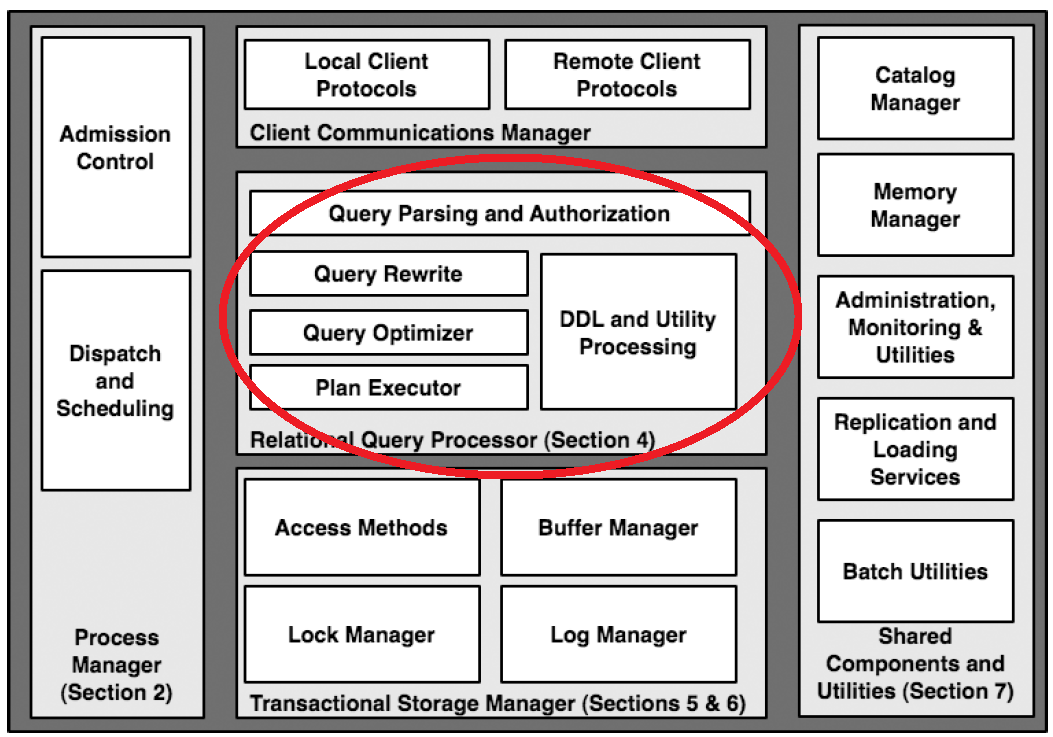
\includegraphics[width=\textwidth,height=0.75\textheight,keepaspectratio]{overall-schema.png} 
\footnote{\tiny{Изображение взято из \cite{Hellerstein2007}}}
\end{figure}
\end{frame}

\begin{frame}
\frametitle{``SELECT... $\rightarrow$ ответ. Как?''}

\begin{figure}[htb]
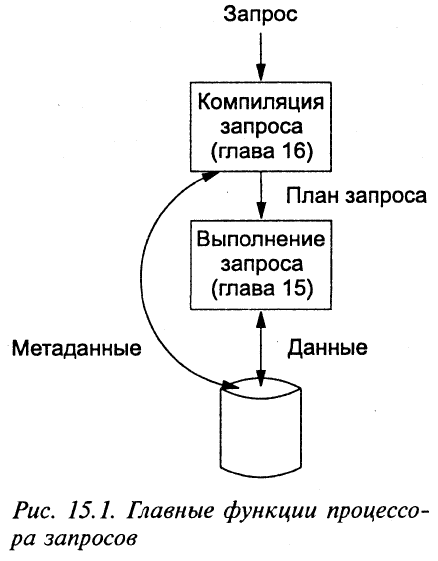
\includegraphics[width=\textwidth,height=0.8\textheight,keepaspectratio]{query-processor.png} 
\footnote{\tiny{Изображение взято из \cite{Ulman2004}}}
\end{figure}

\end{frame}

\begin{frame}
\frametitle{Фаза компиляции запроса}

\begin{figure}[htb]
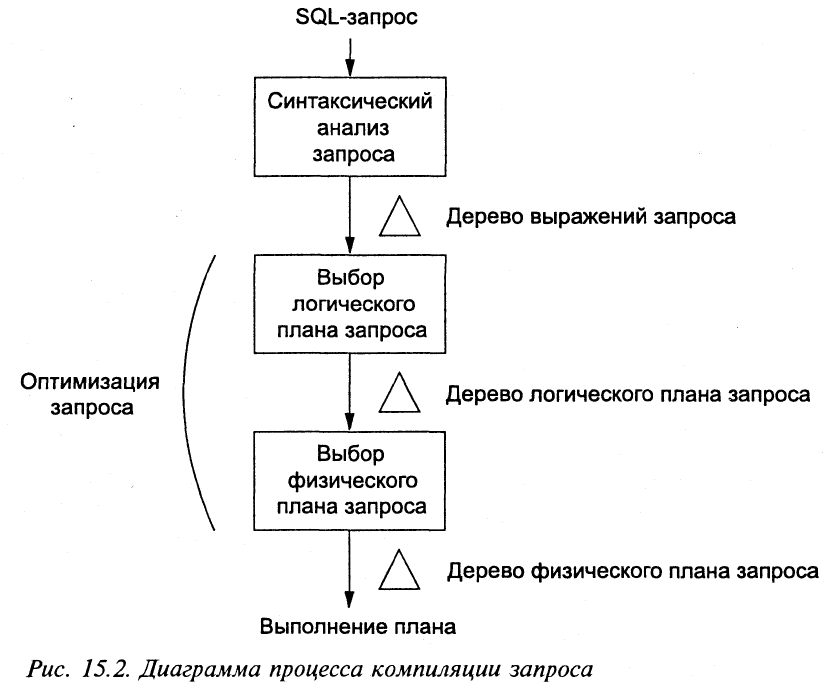
\includegraphics[width=\textwidth,height=0.8\textheight,keepaspectratio]{query-to-execution.png} 
\footnote{\tiny{Изображение взято из \cite{Ulman2004}}}
\end{figure}

\end{frame}

\begin{comment}
\begin{frame}
\frametitle{Шаги компиляции запроса}

Высокоуровнево:

\begin{itemize}
  \setlength\itemsep{1em}
  \item Синтаксический анализ (parsing)~--- построение дерева разбора описывающего структуру запроса;
  \item Перезапись запроса (query rewrite)~--- по дереву разбора строим начальный логический план, затем улучшаем его до эффективного логического плана;
  \item Генерация физического плана (physical plan generation)~--- по логическому плану, на основе метаданных выбираются конкретные реализации операторов.
\end{itemize}
\end{frame}

\end{comment}

\begin{frame}
\frametitle{Фаза компиляции запроса}

\begin{figure}[htb]
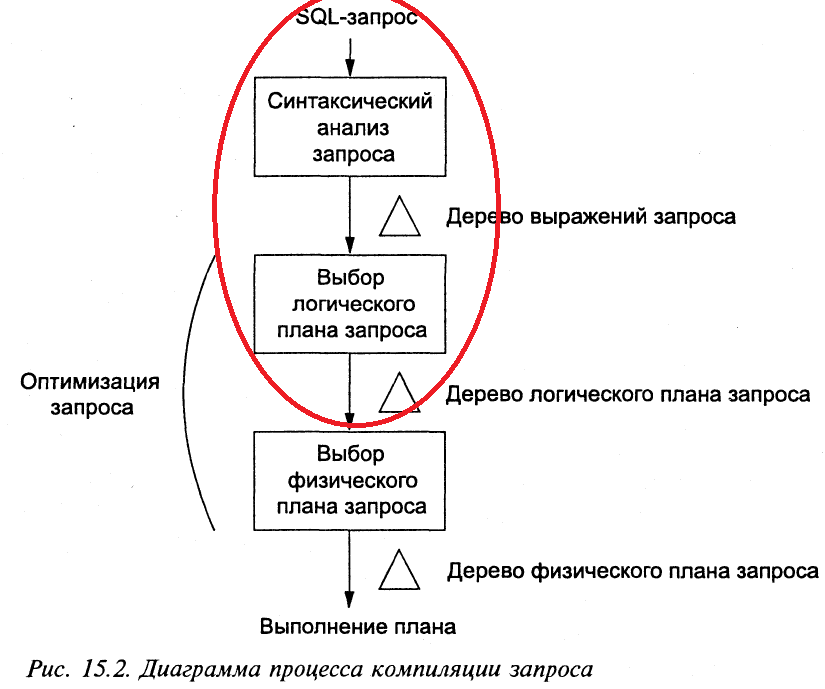
\includegraphics[width=\textwidth,height=0.8\textheight,keepaspectratio]{query-to-execution-circle.png} 
\footnote{\tiny{Изображение взято из \cite{Ulman2004}}}
\end{figure}

\end{frame}

\begin{frame}
\frametitle{От запроса к логическому плану}

\begin{figure}[htb]
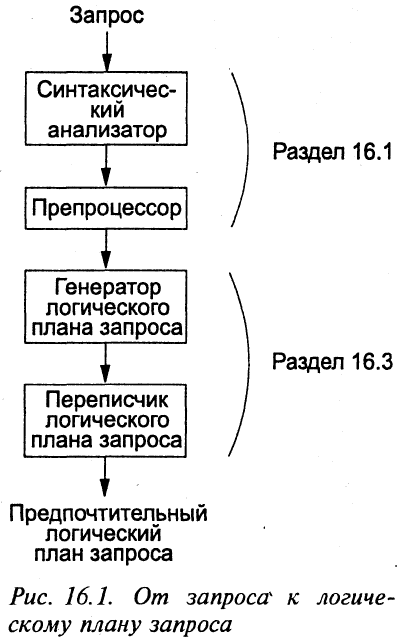
\includegraphics[width=\textwidth,height=0.8\textheight,keepaspectratio]{query-to-logical.png} 
\footnote{\tiny{Изображение взято из \cite{Ulman2004}}}
\end{figure}

\end{frame}

\begin{frame}[allowframebreaks]
\frametitle{Разбор запроса: подробности}

\begin{itemize}
  \setlength\itemsep{1em}
  \item Синтаксический анализ делается достаточно просто, есть масса готовых средств: Flex, Bison, ... . На выходе получается некое внутреннее представление, дерево запроса;
\begin{figure}[htb]
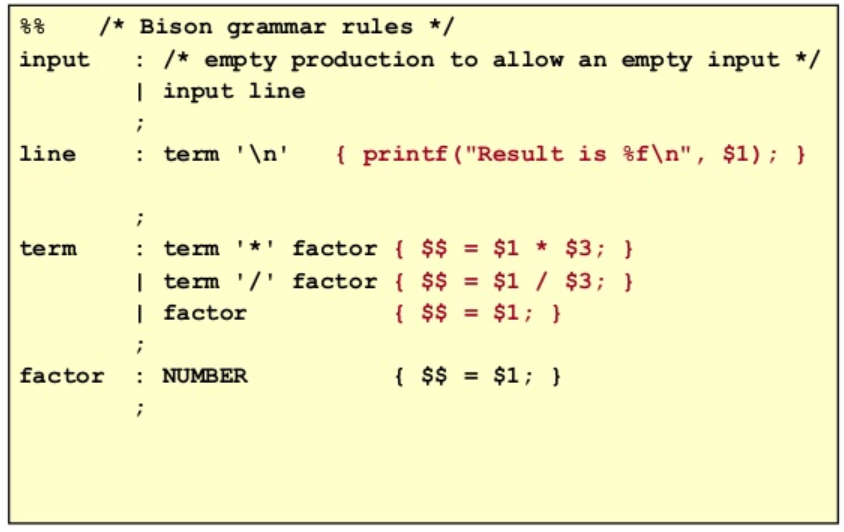
\includegraphics[width=\textwidth,height=0.6\textheight,keepaspectratio]{grammar.png} 
\footnote{\tiny{Изображение взято из \url{https://image.slidesharecdn.com/yacclex-140518211555-phpapp02/95/yacc-lex-11-638.jpg}}}
\end{figure}

  \item Препроцессор~--- подстановка дерева выражений для представлений, разрешение сущностей, семантический контроль:
  \begin{itemize}
    \item Контроль употребления имен отношений;
    \item Контроль использования имен атрибутов и их разрешение;
    \item Контроль типов.
  \end{itemize}  
  \item Фаза перезаписи запроса: упрощение без потери семантики;
  \item Запрос ``собирается'' из набора реляционных операторов, по определенным правилам;
  \item Реляционная алгебра + теоретико-множественные операции позволяют комбинировать эти операторы;
\end{itemize}
Итог: логический план запроса.
\end{frame}

\begin{frame}

\frametitle{Замечания}

В нашей реализации, что будет использоваться на практике, мы будем пользоваться Lemon parser generator.\\~\\

Книга ``Flex \& Bison'' John R. Levine, в 4 главе описывает парсинг для MySQL~--- содержит довольно значительную грамматику и лексер.



\end{frame}

% {Hellerstein2007} --- какие бывают операторы?
% \cite{Taniar2008} --- посмотреть реализации
\begin{frame}
\frametitle{Примеры плана запросов (1)}

\begin{figure}[htb]
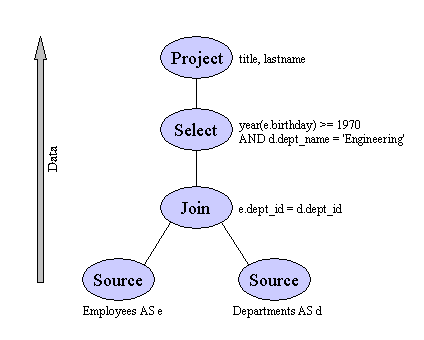
\includegraphics[width=\textwidth,height=0.75\textheight,keepaspectratio]{query-plan1.png} \footnote{\tiny{Изображение взято с https://docs.jboss.org/teiid/6.0/reference/en-US/html/federated\_planning.html}}
\end{figure}
\end{frame}

\begin{frame}
\frametitle{Примеры плана запросов (2)}
\begin{figure}[htb]
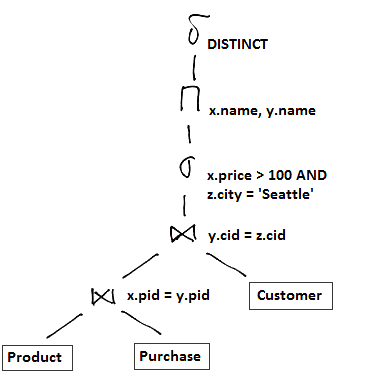
\includegraphics[width=\textwidth,height=0.75\textheight,keepaspectratio]{query-plan2.png} \footnote{\tiny{Изображение взято с http://0agr.ru/wiki/index.php/Logical\_Query\_Plan\_Optimization}}
\end{figure}
\end{frame}

\begin{frame}
\frametitle{Проблемы:}
\begin{itemize}
  \setlength\itemsep{1em}
  \item Планы могут быть очень разные по качеству!
  \item Планов может быть очень много!  
  \item Планы редко когда можно переиспользовать.
  \item ...
\end{itemize}
Вычисление оптимального плана $NP$-трудная задача. Поэтому ищут просто хороший.
\end{frame}

\begin{frame}
\frametitle{Как искать? (1)}

Стоимостная модель + эвристический метод:
\begin{itemize}
  \setlength\itemsep{1em}
  \item Генетические алгоритмы;
  \item Метод симуляции отжига;
  \item Метод восхождения к вершине;
  \item Метод муравьиной оптимизации;
  \item ...
\end{itemize}
На самом деле чаще всего имеется какая-то database-specific процедура перебора планов.
\end{frame}

\begin{frame}
\frametitle{Как искать? (2): иллюстрация}
\begin{figure}[htb]
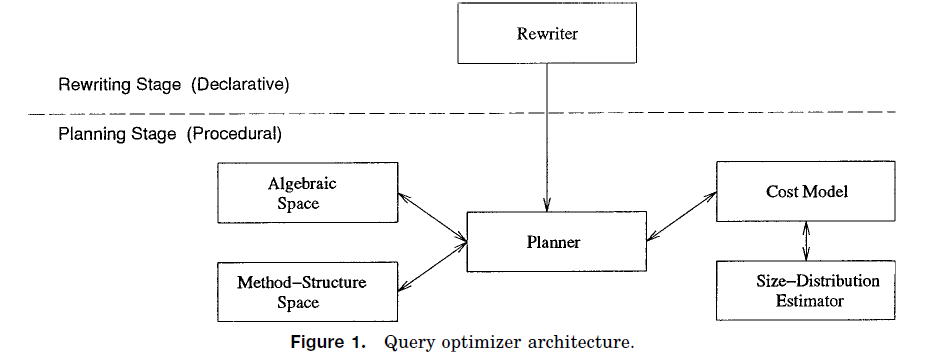
\includegraphics[width=\textwidth,height=0.7\textheight,keepaspectratio]{overall-schema2.png} 
\footnote{\tiny{Изображение взято из \cite{Ioannidis1996}}}
\end{figure}
\end{frame}

\begin{frame}
\frametitle{Итераторная модель Volcano}

Пусть у нас есть план, надо его запустить на выполнение.

\begin{figure}[htb]
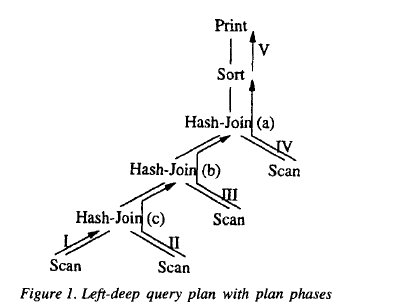
\includegraphics[width=\textwidth,height=0.7\textheight,keepaspectratio]{plan.png} 
\footnote{\tiny{Изображение взято из \cite{Graefe1996}}}
\end{figure}

\end{frame}

\begin{frame}[fragile]
\frametitle{Итератор}

\lstset{language=C++}
\begin{lstlisting}
class AbstractNode{
     private:
         AbstractNode* LChild;
         AbstractNode* RChild;	
         void* ...	// internal state
     public:
         int Open();
         int Close();
         void* GetNext();
};
\end{lstlisting}
\begin{itemize}
  \item Идея: строим дерево из таких итераторов;
  \item Его можно запускать, вызывая у верхнего оператора GetNext();
  \item Обычно, между операторами ходит не одна, а много записей (блочная модель Volcano).
\end{itemize}

\end{frame}

\begin{frame}[fragile]
\frametitle{Материализация и пайплайнинг}

Сколько записей должно быть в блоке?
\begin{itemize}
    \setlength\itemsep{1em}
	\item Крайний случай: все~--- полная материализация;
	\item Крайний случай: одна~--- пайплайнинг в стиле начала нулевых;
	\item Что-то посередине.
\end{itemize}

Как выбирать? 
	 
\begin{itemize}
	\setlength\itemsep{1em}
	\item Зависит от аппаратных параметров: e.g. размера кеша на машине; 
	\item Зависит от программных параметров: e.g. сколько памяти отдается на запрос;
	\item Зависит от нагрузки: сколько и каких запросов предполагается обрабатывать одновременно;
	\item Наконец, зависит от типа системы.
\end{itemize}

\end{frame}

\begin{frame}
\frametitle{Примеры простых итераторов}

\begin{figure}[htb]
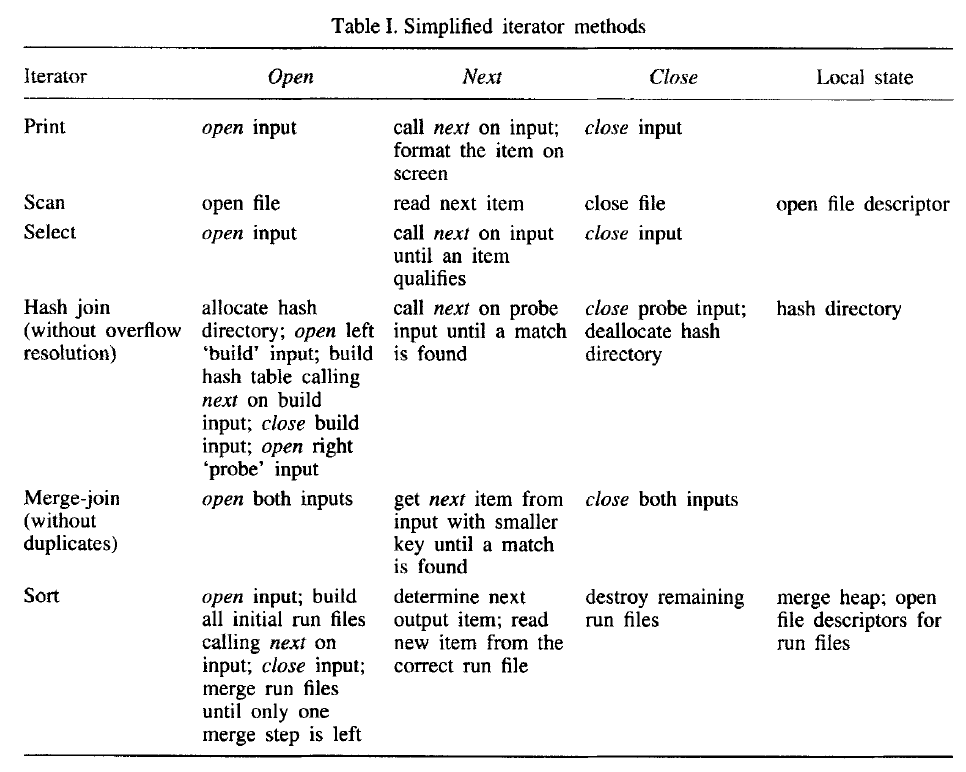
\includegraphics[width=\textwidth,height=0.8\textheight,keepaspectratio]{iterators.png} 
\footnote{\tiny{Изображение взято из \cite{Graefe1996}}}
\end{figure}

\end{frame}

\begin{comment}

\begin{frame}
\frametitle{Данные на диске}

В двух словах (очень приблизительно):

\begin{itemize}
  \setlength\itemsep{1em}
  \item Данных хранятся на диске;
  \item Считываются и \alert{временно} хранятся в памяти;
  \item Обычно какой-то memory mapping;
  \item Буфер-менджер: считывание, удержание в памяти, модификация данных, сброс на диск;
  \item ``Нарезка'' на страницы: единицы оперирования буфер-менеджера;
\end{itemize}

Как представлять страницу? Записи ведь бывают переменной длины!

\end{frame}

\begin{frame}
\frametitle{Слотированная страница}

\begin{figure}[htb]
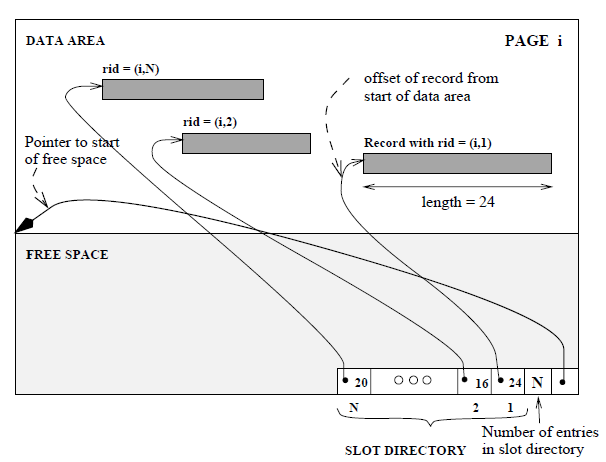
\includegraphics[width=\textwidth,height=0.8\textheight,keepaspectratio]{slotted.png} 
\footnote{\tiny{Изображение взято из \cite{Ramakrishnan2000}}}
\end{figure}

\end{frame}

\end{comment}


\begin{frame}
\frametitle{Реализация операторов}

Нужен минимальный набор:

\begin{itemize}
  \item $(\sigma)$ Выборка~--- то, что содержится во WHERE: T1.X > 255;
  \item $(\bowtie)$ Соединение~--- бывает:
  \begin{itemize}
    \item во WHERE: T1.X = T2.Y и,
    \item в FROM: FROM Orders INNER JOIN Customers ON Orders.CustomerID=Customers.CustomerID
  \end{itemize}
  \item $(\sqcap)$ Проекция~--- остается то, что содержится в SELECT: SELECT Orders.OrderID, Customers.CustomerName
\end{itemize}

Такой класс запросов называется SPJ запросы (Select, Project, Join).\\~\\

Это самый простой класс, есть еще операторы: агрегация, DISTINCT, TOP N, множественные операции (UNION, MINUS, ...), подзапросы, ...

\end{frame}


\begin{frame}
\frametitle{Реализация выборки}

Реализация выборки = методы доступа (access methods). 
\\~\\
Основные:

\begin{itemize}
  \item Полный просмотр~--- медленный, но не требует ничего дополнительно, данные-то всяко есть;
  \item Просмотр по кластеризованному индексу~--- быстрый, но можно только по одной комбинации атрибутов;
  \item Просмотр с использованием индекса~--- быстрый, можно по любому количеству комбинаций атрибутов, но надо строить.
\end{itemize}

Сложные: например, по нескольким индексам, пересечение и вычитка.

\end{frame}

\begin{frame}
\frametitle{Напоминание про индекс на B-tree}

\begin{figure}[htb]
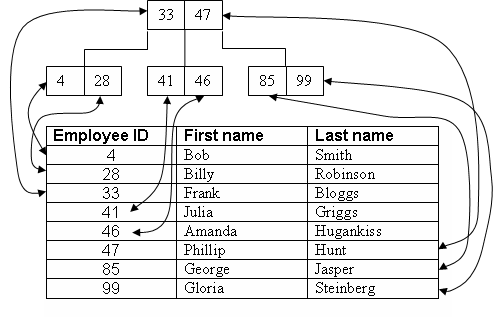
\includegraphics[width=\textwidth,height=0.8\textheight,keepaspectratio]{btree-index.png} 
\footnote{\tiny{Изображение взято из \url{https://upload.wikimedia.org/wikipedia/en/0/03/Btree\_index.PNG}}}
\end{figure}

\end{frame}




\begin{frame}
\frametitle{Реализация реляционной операции соединение}

\begin{columns}
  \begin{column}{0.5\textwidth}
    \begin{table}
      \begin{tabular}{ l | l | l | l | c }
        id & name & wage & skill & roomid \\
        1 & ivan & 80 & c++ & 1 \\  
        2 & petr & 50 & c++ & 1 \\
        3 & slava & 30 & java & 3 \\
        4 & vasya & 60 & php & 2 \\
        5 & sasha & 70 & java & 2 \\
      \end{tabular}
      \caption{wages}
    \end{table}
  \end{column}

  \begin{column}{0.5\textwidth}
    \begin{table}
      \begin{tabular}{ l | l | l | c  }
        id & name & screen & floor \\
        1 & 401 & 14 & 4 \\  
        2 & 303 & 30 & 3 \\
        3 & 302 & 24 & 3 \\
      \end{tabular}
      \caption{rooms}
    \end{table}
  \end{column}
\end{columns}

Основные методы: Nested Loop, Sort-Merge, Hash-Join.\\~\\

\alert{В следующих слайдах обращайте внимание на отсортированность атрибутов!}

\end{frame}

\setbeamercovered{invisible}

\begin{frame}
\frametitle{Nested Loop}

\onslide<1->

\begin{columns}
  \begin{column}{0.5\textwidth}
    \begin{table}
      \begin{tabular}{ l | l | l | l | c }
        id & name & wage & skill & roomid \\
        1 & ivan & 80 & c++ & \only<1,2,3>{\tikz[baseline,remember picture]{\node[fill=green!20,anchor=base] (t1){1};}}\only<4->{1} \\  
        2 & petr & 50 & c++ & \only<4,5,6>{\tikz[baseline,remember picture]{\node[fill=green!20,anchor=base] (t2){1};}}\only<1,2,3,7->{1} \\
        3 & slava & 30 & java &  \only<7,8,9>{\tikz[baseline,remember picture]{\node[fill=green!20,anchor=base] (t3){3};}}\only<1,2,3,4,5,6,10->{3} \\
        4 & vasya & 60 & php & \only<10,11,12>{\tikz[baseline,remember picture]{\node[fill=green!20,anchor=base] (t4){2};}}\only<1,2,3,4,5,6,7,8,9,13->{2} \\
        5 & sasha & 70 & java & \only<13,14,15>{\tikz[baseline,remember picture]{\node[fill=green!20,anchor=base] (t5){2};}}\only<1,2,3,4,5,6,7,8,9,10,11,12>{2} \\
      \end{tabular}
      \caption{wages}
    \end{table}
  \end{column}

  \begin{column}{0.5\textwidth}
    \begin{table}
      \begin{tabular}{ c | l | l | c  }
        id & name & screen & floor \\
        \only<1,4,7,10,13>{\tikz[baseline,remember picture]{\node[fill=red!20,anchor=base] (n1){1};}} \only<2,3,5,6,8,9,11,12,14,15>{1} & 401 & 14 & 4 \\  
        \only<2,5,8,11,14>{\tikz[baseline,remember picture]{\node[fill=red!20,anchor=base] (n2){3};}} \only<1,3,4,6,7,9,10,12,13,15>{3} & 303 & 30 & 3 \\
        \only<3,6,9,12,15>{\tikz[baseline,remember picture]{\node[fill=red!20,anchor=base] (n3){2};}} \only<1,2,4,5,7,8,10,11,13,14>{2} & 302 & 24 & 3 \\
      \end{tabular}
      \caption{rooms}
    \end{table}
  \end{column}
\end{columns}

\begin{tikzpicture}[remember picture,overlay]   %% use here too
    \only<1>{\path[very thick,->] (t1) edge (n1);}
    \only<2>{\path[very thick,->] (t1) edge (n2);}
    \only<3>{\path[very thick,->] (t1) edge (n3);}   

    \only<4>{\path[very thick,->] (t2) edge (n1);}
    \only<5>{\path[very thick,->] (t2) edge (n2);}
    \only<6>{\path[very thick,->] (t2) edge (n3);}   

    \only<7>{\path[very thick,->] (t3) edge (n1);}
    \only<8>{\path[very thick,->] (t3) edge (n2);}
    \only<9>{\path[very thick,->] (t3) edge (n3);}          

    \only<10>{\path[very thick,->] (t4) edge (n1);}
    \only<11>{\path[very thick,->] (t4) edge (n2);}
    \only<12>{\path[very thick,->] (t4) edge (n3);}          

    \only<13>{\path[very thick,->] (t5) edge (n1);}
    \only<14>{\path[very thick,->] (t5) edge (n2);}
    \only<15>{\path[very thick,->] (t5) edge (n3);}                    
                  
\end{tikzpicture}

\texttt{Выдача: \only<1,2,3>{1-1} \only<4,5,6,7>{1-1, 2-1} \only<8,9,10,11>{1-1, 2-1, 3-2} \only<12,13,14>{1-1, 2-1, 3-2, 4-3} \only<15>{1-1, 2-1, 3-2, 4-3,5-3}}

\end{frame}

\begin{frame}
\frametitle{Sort-Merge}

\onslide<1->

\begin{columns}
  \begin{column}{0.5\textwidth}
    \begin{table}
      \begin{tabular}{ l | l | l | l | c }
        id & name & wage & skill & roomid \\
        1 & ivan & 80 & c++ & \only<1>{\tikz[baseline,remember picture]{\node[fill=green!20,anchor=base] (t1){1};}}\only<2->{1} \\  
        2 & petr & 50 & c++ & \only<2>{\tikz[baseline,remember picture]{\node[fill=green!20,anchor=base] (t2){1};}}\only<1,3->{1} \\
        4 & vasya & 60 & php & \only<3>{\tikz[baseline,remember picture]{\node[fill=green!20,anchor=base] (t3){2};}}\only<1,2,4->{2} \\
        5 & sasha & 70 & java & \only<4>{\tikz[baseline,remember picture]{\node[fill=green!20,anchor=base] (t4){2};}}\only<1,2,3,5->{2} \\
        3 & slava & 30 & java & \only<5>{\tikz[baseline,remember picture]{\node[fill=green!20,anchor=base] (t5){3};}}\only<1,2,3,4>{3} \\
        
      \end{tabular}
      \caption{wages}
    \end{table}
  \end{column}

  \begin{column}{0.5\textwidth}
    \begin{table}
      \begin{tabular}{ c | l | l | c  }
        id & name & screen & floor \\
        \only<1,2>{\tikz[baseline,remember picture]{\node[fill=red!20,anchor=base] (n1){1};}} \only<3->{1} & 401 & 14 & 4 \\  
        \only<3,4>{\tikz[baseline,remember picture]{\node[fill=red!20,anchor=base] (n2){2};}} \only<1,2,5>{2} & 302 & 24 & 3 \\       
        \only<5>{\tikz[baseline,remember picture]{\node[fill=red!20,anchor=base] (n3){3};}} \only<1,2,3,4>{3} & 303 & 30 & 3 \\
      \end{tabular}
      \caption{rooms}
    \end{table}
  \end{column}
\end{columns}

\begin{tikzpicture}[remember picture,overlay]   %% use here too
    \only<1>{\path[very thick,<->] (t1) edge (n1);}
    \only<2>{\path[very thick,<->] (t2) edge (n1);}
    \only<3>{\path[very thick,<->] (t3) edge (n2);}
    \only<4>{\path[very thick,<->] (t4) edge (n2);}
    \only<5>{\path[very thick,<->] (t5) edge (n3);}
\end{tikzpicture}

\texttt{Выдача: \only<1>{1-1} \only<2>{1-1, 2-1} \only<3>{1-1, 2-1, 3-2} \only<4>{1-1, 2-1, 3-2, 4-3} \only<5>{1-1, 2-1, 3-2, 4-3,5-3}}

\end{frame}

\begin{frame}
\frametitle{Hash-Join}
\only<1,2,3>{\center{Фаза хеширования}}\only<4->{\center{Фаза пробинга}}

\begin{columns}
  \begin{column}{0.5\textwidth}
    \begin{table}
      \begin{tabular}{ l | l | l | l | c }
        id & name & wage & skill & roomid \\
        1 & ivan & 80 & c++ & \only<4>{\tikz[baseline,remember picture]{\node[fill=green!20,anchor=base] (t1){1};}}\only<1,2,3,5->{1} \\  
        2 & petr & 50 & c++ & \only<5>{\tikz[baseline,remember picture]{\node[fill=green!20,anchor=base] (t2){1};}}\only<1,2,3,4, 6->{1} \\
        3 & slava & 30 & java & \only<6>{\tikz[baseline,remember picture]{\node[fill=green!20,anchor=base] (t3){3};}}\only<1,2,3,4,5,7->{3} \\
        4 & vasya & 60 & php & \only<7>{\tikz[baseline,remember picture]{\node[fill=green!20,anchor=base] (t4){2};}}\only<1,2,3,4,5,6,8->{2} \\
        5 & sasha & 70 & java & \only<8>{\tikz[baseline,remember picture]{\node[fill=green!20,anchor=base] (t5){2};}}\only<1,2,3,4,5,6,7>{2} \\
      \end{tabular}
      \caption{wages}
    \end{table}
  \end{column}

  \begin{column}{0.5\textwidth}
    \begin{table}
      \begin{tabular}{ c | l | l | c  }
        id & name & screen & floor \\
        \only<1>{\tikz[baseline,remember picture]{\node[fill=red!20,anchor=base] (n1){1};}} \only<2->{1} & 401 & 14 & 4 \\  
        \only<2>{\tikz[baseline,remember picture]{\node[fill=red!20,anchor=base] (n2){3};}} \only<1,3->{3} & 303 & 30 & 3 \\
        \only<3>{\tikz[baseline,remember picture]{\node[fill=red!20,anchor=base] (n3){2};}} \only<1,2,4->{2} & 302 & 24 & 3 \\
      \end{tabular}
      \caption{rooms}
    \end{table}
  \end{column}
\end{columns}
Хеш: \onslide<1>{1}\onslide<2>{1, 3}\onslide<3->{\tikz[baseline,remember picture]{\node[fill=blue!20,anchor=base] (h1){1};}, \tikz[baseline,remember picture]{\node[fill=blue!20,anchor=base] (h2){2};}, \tikz[baseline,remember picture]{\node[fill=blue!20,anchor=base] (h3){3};}}

Выдача: \only<4>{1-1} \only<5>{1-1, 2-1} \only<6>{1-1, 2-1, 3-2} \only<7>{1-1, 2-1, 3-2, 4-3} \only<8>{1-1, 2-1, 3-2, 4-3,5-3}

\begin{tikzpicture}[remember picture,overlay]   %% use here too
    \only<3->{\path[very thick,->] (h1) edge (n1);}
    \only<3->{\path[very thick,->] (h2) edge (n3);}
    \only<3->{\path[very thick,->] (h3) edge (n2);}
\end{tikzpicture}

\end{frame}


\begin{frame}
\frametitle{Проекция}

\begin{itemize}
  \setlength\itemsep{1em}
  \item Обычно стараются делать сразу, как только возможно;
  \item Часто прячут внутрь других операторов;
\end{itemize}

\end{frame}

\begin{frame}
\frametitle{Агрегация: напоминание}
\begin{table}
  \begin{tabular}{ l | l | l | l | c }
    id & name & wage & skill & exp \\
    1 & ivan & 80 & c++ & 5 \\  
    2 & petr & 50 & c++ & 3 \\
    3 & slava & 30 & java & 1 \\
    4 & vasya & 60 & php & 1 \\
    5 & sasha & 70 & java & 3 \\
    6 & dasha & 65 & c++ & 3 \\
    7 & katya & 50 & java & 1 \\        
    8 & glasha & 30 & bash & 2 \\
    9 & oleg & 20 & php & 3 \\    
    10 & boris & 50 & java & 3 \\    
  \end{tabular}
  \caption{wages}
\end{table}

SELECT skill, avg(wage), exp FROM wages GROUP BY skill, exp

\end{frame}

\begin{frame}
\frametitle{Агрегация: как?}
\begin{itemize}
  \item Влоб: завести набор групп, сверяться каждый раз со всеми; 
  \item Отсортировать по GROUP BY, а потом аккуратно пройтись один раз.
\end{itemize}

Упражнения: 

\begin{itemize}
  \item Что выдаст запрос?
  \item Расписать как будет происходить вычисление.
\end{itemize}
\end{frame}


\begin{frame}
\frametitle{Замечание о порядках сортировки}
\begin{itemize}
  \setlength\itemsep{1em}
  \item Они очень сильно помогают;
  \item Каждый раз при запросе пересортировывать~--- долго;
  \item Сделать пресортировку один раз, по этому атрибуту. Однако, на диске таблицу держать в отсортированном виде можно только по одному атрибуту.
\end{itemize}
\end{frame}

\begin{frame}
\frametitle{Замечание про операторы}
\footnotesize
Операторы бывают:
\begin{itemize}  
  \item Блокирующие, например hash-join или сканирование с сортировкой;
  \item Не блокирующие.
\end{itemize}

А еще они могут ломать сортировку или нет:
\begin{itemize}  
  \item Sort-merge join сохраняет сортировку по обоим атрибутам;
  \item Hash join испортит по одному атрибуту.
\end{itemize}

%Сортировка может очень пригодиться в других оперторах :(

Операторы можно параллелить, как по-отдельности, так и внутри:

\begin{figure}[htb]
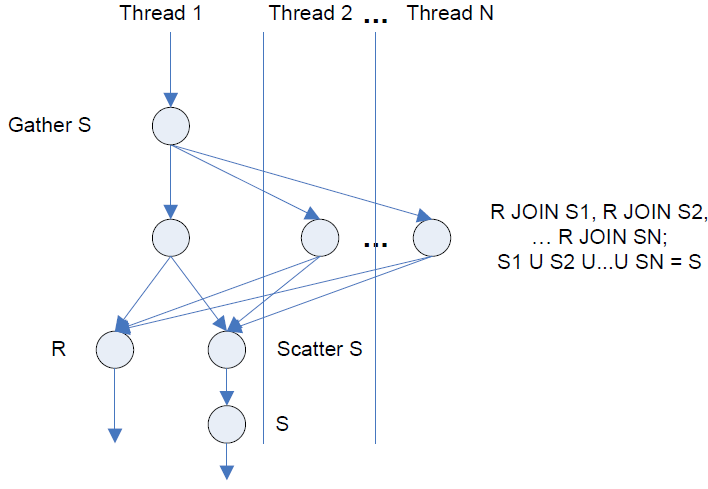
\includegraphics[width=\textwidth,height=0.30\textheight,keepaspectratio]{parallel.png} 
\end{figure}

Более подробно смотри \cite{Taniar2008}.

\end{frame}

\begin{frame}
\frametitle{Современность и альтернативы: компиляция запросов I}

	То, что рассматривалось выше (Volcano) называется \alert{интерпретацией} запросов. А бывает еще и \alert{компиляция} запросов в код и она очень популярна сейчас, фактически баззворд.
	
	\begin{itemize}
		\setlength\itemsep{1em}
		\item Пытались так делать с 80х, но дело не пошло: долго компилируется, да и сейчас заметные затраты;
		\item Сейчас (2010+) компиляция есть очень во многих индустриальных системах, в 10х был бум исследований;
		\item Кажется что для дисковых систем подход не особо важен;
		\item Из разговоров разработчиками крупных систем: 
		\begin{itemize}
			\item очень тяжело разрабатывать и мейнтейнить такие системы;
			\item а выгода-то не такая уж и заметная, на отдельных запросах до 30\%
		\end{itemize}	
	\end{itemize}
	
	Итог: кажется что овчинка стоит выделки только при проверке предикатов. Но и тут у подхода есть конкуренты (e.g. стековые машины).
\end{frame}

\begin{frame}[fragile]
	\frametitle{Современность и альтернативы: компиляция запросов II}

	\begin{columns}
		\begin{column}{0.48\textwidth}
			\begin{figure}[htb]
			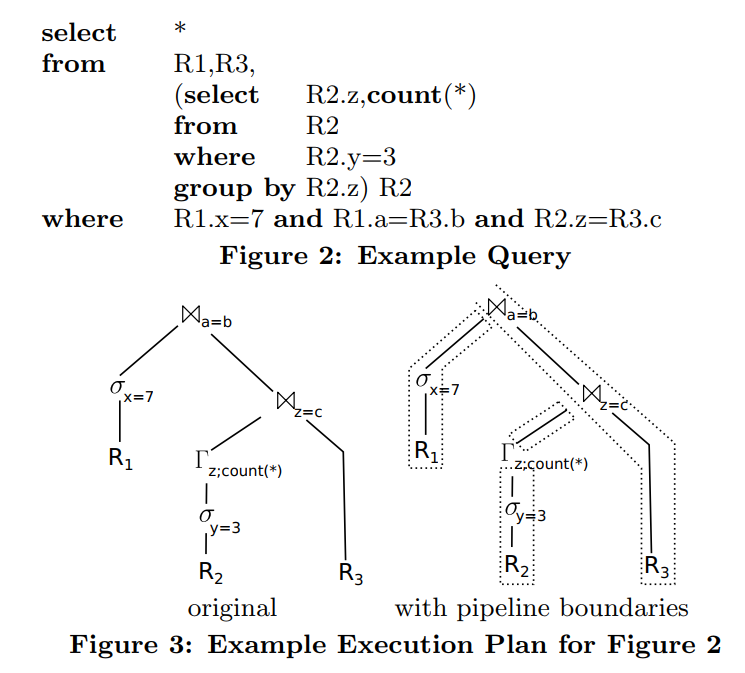
\includegraphics[width=\textwidth,height=0.40\textheight,keepaspectratio]{compilation-2.png} 
			\end{figure}
		\end{column}
		\begin{column}{0.48\textwidth}
			\begin{figure}[htb]
			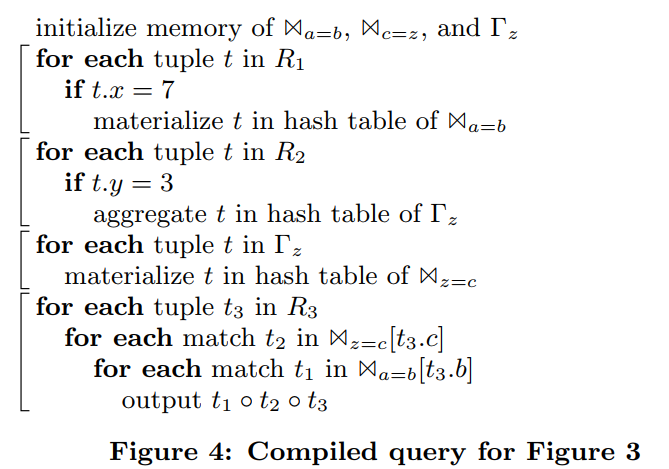
\includegraphics[width=\textwidth,height=0.40\textheight,keepaspectratio]{compilation-3.png} 
			\end{figure}
		\end{column}
	\end{columns}

	\begin{figure}[htb]
		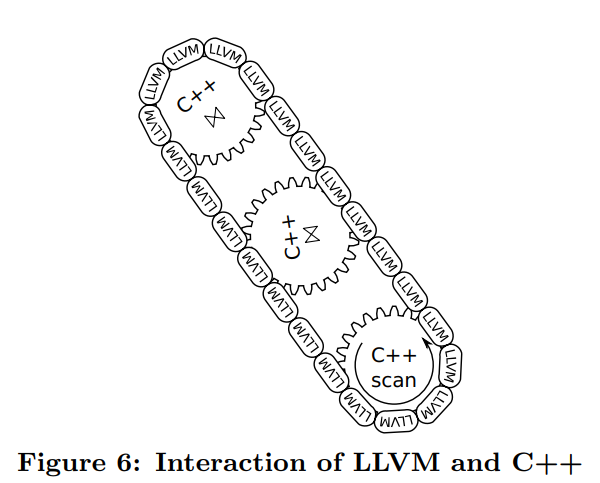
\includegraphics[width=\textwidth,height=0.30\textheight,keepaspectratio]{compilation-1.png}\footnote{\tiny{Все изображение на этом слайде взяты из \cite{Neumann2011}}}
	\end{figure}
	
\end{frame}

\begin{frame}[fragile]
	\frametitle{Современность и альтернативы: компиляция запросов III}
	Как генерировать код? Авторы попробовали генерировать C++ код но это оказалось долго и неудобно: сложный запрос компилировался несколько секунд. 
	\\~\\
	Пришли к связке \underline{прекомпилированных C++ кусочков} (реализация сложных компонентов) и \underline{генерация в LLVM ассемблер}, который JIT компилировался и вызывал C++ кусочки.
	\begin{figure}[htb]
		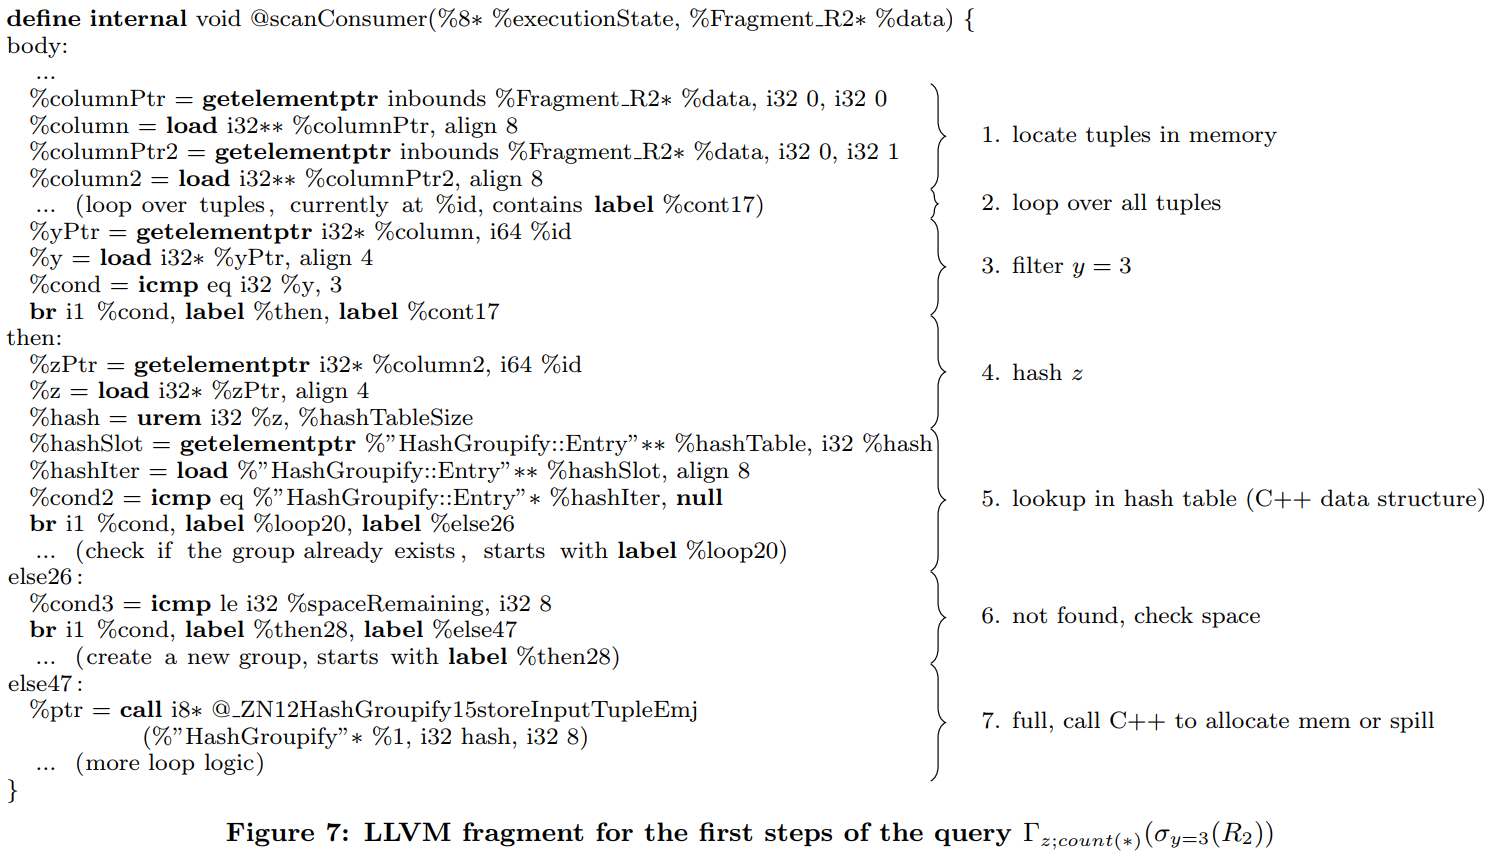
\includegraphics[width=\textwidth,height=0.40\textheight,keepaspectratio]{compilation-4.png}\footnote{\tiny{Все изображение на этом слайде взяты из \cite{Neumann2011}}}
	\end{figure}
	
\end{frame}

\begin{frame}[fragile]
	\frametitle{Современность и альтернативы: push-based модели}
	Сейчас есть два понимания push-based моделей: интерпретационные и компиляционные. Мы говорим сейчас о первых!

	\begin{itemize}
		\item Идея: оператор живет в своем потоке и нотифицирует родителя о том, что результат готов;
		\item Тяжелее в реализации, требуют большого количества ядер;
		\item Иногда без них не обойтись: могут решить проблему ромба в потоках данных;
		\item Не знаю индустриальных систем где бы использовался $\longrightarrow$ сейчас представляют только исследовательский интерес:
		\begin{itemize}
			\item Переиспользование промежуточных результатов: QPipe~\cite{qpipe1}, \cite{qpipe2} и другие системы \cite{sharing1}, \cite{sharing2};
			\item Адаптивность (изменение плана или способа выполнения находу): Eddies~\cite{eddies}
		\end{itemize}
		
	\end{itemize}
	
\end{frame}

\begin{frame}[allowframebreaks]
	\frametitle{Современность и альтернативы: как, что устроено}
	\scriptsize
	
\begin{table}	
	
\begin{longtable}{|p{2cm}|c|c|c|p{2.5cm}|p{1cm}|}
	\hline
	Название & год  & тип  & pull/push  & t/b/op-at-a-time  & source \\
	\hline
	
	PostgreSQL & 1996 & D & pull & tuple & link\footnote{\url{
		http://citeseerx.ist.psu.edu/viewdoc/download?doi=10.1.1.357.4302&rep=rep1&type=pdf }}\\


	SQLite & 2000 & M & pull & tuple & link\footnote{\url{
		https://dbdb.io/db/sqlite }}\\	
	
	MariaDB & pre-2019  & D & none  & ? & link\footnote{\url{winand.at/newsletter/2019-12/partiql-microsoft-licenses-volcano-model }} \\
	
	MariaDB & 2019  & D & pull  & ? & link\footnote{\url{https://dev.mysql.com/worklog/task/?id=11785\#tabs-11785-4}} \\
	
	CockroachDB & 2015 & ? & pull & block & link\footnote{\url{ https://dbdb.io/db/cockroachdb}}\\
	
	
	Vertica & 2005 & D & оба? & ? & link\footnote{\url{
			https://www.vertica.com/kb/Reading-Query-Plans/Content/BestPractices/Reading-Query-Plans.htm}} \\ 
		
	\hline
	
	SYBASE Adaptive Server Enterprise 15.5 & 1987 & D & pull & tuple & link\footnote{\url{
			http://infocenter.sybase.com/help/topic/com.sybase.infocenter.dc00743.1502/html/queryprocessing/queryprocessing1.htm 
	}}\\

	\hline


	SAP HANA & 2010 & M & ? & block & link\footnote{\url{https://dbdb.io/db/sap-hana 
	}}\\


	
	Snowflake & 2014 & D? & push & block & link\footnote{\url{https://dbdb.io/db/snowflake 
	}}\\

	\hline


	Microsoft SQL Server Hekaton Engine & 2014 & M & компиляция (pull?) & tuple? & link\footnote{Compilation in the Microsoft SQL Server Hekaton Engine}\\
	
	\hline
	
	
	HyPer & $\approxeq 2006$ & M & компиляция (push) & ? & link\footnote{Franz Faerber et al. (2017), "Main Memory Database Systems", Foundations and Trends® in Database}, link\footnote{\url{https://15721.courses.cs.cmu.edu/spring2018/notes/03-compilation.pdf}}, link\footnote{Building Efficient Query Engines in a High-Level Language}\\
	

	

	
	
	\hline
\end{longtable}

\end{table}	

\end{frame}


\begin{frame}[allowframebreaks]
\frametitle{Ссылки}
\footnotesize{
\begin{thebibliography}{99}

\bibitem[Garcia-Molina et al., 2004] {Ulman2004} Гектор Гарсиа-Молина, Джеффри Д. Ульман, Дженнифер Уидом. Системы баз данных. Полный курс.  ISBN 5-8459-0384-Х; 2004 г. 

\bibitem[Hellerstein et al., 2007] {Hellerstein2007} Joseph M. Hellerstein, Michael Stonebraker, and James Hamilton. 2007. Architecture of a Database System. Found. Trends databases 1, 2 (February 2007), 141--259. 

\bibitem[Ioannidis, 1996] {Ioannidis1996} Yannis E. Ioannidis. 1996. Query optimization. ACM Comput. Surv. 28, 1 (March 1996), 121--123. DOI=http://dx.doi.org/10.1145/234313.234367 

\bibitem[Smirnov and Chernishev, 2011] {Smirnov2011} Kirill Smirnov and George Chernishev. Benchmarking Inter and Intra Operator Parallelism on Contemporary Desktop Hardware. In Proc. of SYRCoDIS 2011, p. 62--67, 2011.

\bibitem[Graefe, 1996] {Graefe1996} Goetz Graefe. 1996. Iterators, schedulers, and distributed-memory parallelism. Softw. Pract. Exper. 26, 4 (April 1996), 427--452. DOI=http://dx.doi.org/10.1002/(SICI)1097-024X(199604)26:4<427::AID-SPE20>3.3.CO;2-8 

\bibitem[Taniar et al., 2008] {Taniar2008} David Taniar, Clement H. C. Leung, Wenny Rahayu, and Sushant Goel. 2008. High Performance Parallel Database Processing and Grid Databases. Wiley Publishing. 

\bibitem[Ramakrishnan and Gehrke, 2000] {Ramakrishnan2000}  Raghu Ramakrishnan and Johannes Gehrke. 2000. Database Management Systems (2nd ed.). Osborne/McGraw-Hill, Berkeley, CA, USA. 

\bibitem[Avnur and Hellerstein, 2000] {eddies} Avnur, R., Hellerstein, J.M.: Eddies: continuously adaptive query processing. Proc. SIGMOD 2000, 261–272 (2000)

\bibitem[Harizopoulos et al., 2005] {qpipe1} Stavros Harizopoulos, Vladislav Shkapenyuk, and Anastassia Ailamaki. QPipe: a simultaneously pipelined relational query engine. SIGMOD ’05

\bibitem[Psaroudakis et al, 2014] {qpipe2} Iraklis Psaroudakis, Manos Athanassoulis, Matthaios Olma, and Anastasia Ailamaki. 2014. Reactive and proactive sharing across concurrent analytical queries. SIGMOD ’14

\bibitem[Makreshanski et al, 2018] {sharing1} Darko Makreshanski, Georgios Giannikis, Gustavo Alonso, and Donald Kossmann. 2018. Many-query join: efficient shared execution of relational joins on modern hardware. The VLDB Journal 27, 5 (October   2018), 669–692.

\bibitem[Arumugam et al, 2010] {sharing2} Subi Arumugam et al. 2010. The DataPath system: a data-centric analytic processing engine for large data warehouses. In Proceedings of the 2010 ACM SIGMOD International Conference on Management of data (SIGMOD ’10). Association for Computing Machinery, New York, NY, USA, 519–530.

\bibitem[T. Neumann, 2011] {Neumann2011} Neumann. Efficiently Compiling Efficient Query Plans for Modern Hardware. PVLDB, 4(9):539–550, 2011.


\end{thebibliography}
}
\end{frame}


\end{document} 